% Journal Article
% LaTeX Template
%----------------------------------------------------------------------------------------
%	PACKAGES AND OTHER DOCUMENT CONFIGURATIONS
%----------------------------------------------------------------------------------------

\documentclass[twoside,twocolumn]{article}

\usepackage{blindtext} % Package to generate dummy text throughout this template 

\usepackage[sc]{mathpazo} % Use the Palatino font
\usepackage[T1]{fontenc} % Use 8-bit encoding that has 256 glyphs
\linespread{1.05} % Line spacing - Palatino needs more space between lines
\usepackage{microtype} % Slightly tweak font spacing for aesthetics

\usepackage[english]{babel} % Language hyphenation and typographical rules
\usepackage{graphicx}
\usepackage{amsmath}
\usepackage{amssymb}
\DeclareMathOperator{\Tr}{Tr}
\usepackage[hmarginratio=1:1,top=32mm,columnsep=20pt]{geometry} % Document margins
\usepackage[format=plain, small,labelfont=bf,up,textfont=it,up]{caption} 
\usepackage{booktabs} % Horizontal rules in tables

\usepackage{lettrine} % The lettrine is the first enlarged letter at the beginning of the text
\usepackage{units}

\usepackage{enumitem} % Customized lists
\setlist[itemize]{noitemsep} % Make itemize lists more compact

\usepackage{abstract} % Allows abstract customization
\renewcommand{\abstractname}{\vspace{-\baselineskip}}
\renewcommand{\abstractnamefont}{\normalfont\bfseries} % Set the "Abstract" text to bold
% Set the abstract itself to small italic text
\renewcommand{\abstracttextfont}{\normalfont\small\itshape} 

\usepackage{titlesec} % Allows customization of titles
\renewcommand\thesection{\Roman{section}} % Roman numerals for the sections
\renewcommand\thesubsection{\roman{subsection}} % roman numerals for subsections
% Change the look of the section titles
\titleformat{\section}[block]{\large\scshape\centering}{\thesection.}{1em}{}
% Change the look of the section titles
\titleformat{\subsection}[block]{\large}{\thesubsection.}{1em}{}

\usepackage{fancyhdr} % Headers and footers
\pagestyle{fancy} % All pages have headers and footers
\fancyhead{} % Blank out the default header
\fancyfoot{} % Blank out the default footer
% Custom header text
\fancyhead[C]{Qiskit $\bullet$ April 2020} % $\bullet$ Vol. XXI, No. 1}
\fancyfoot[RO,LE]{\thepage} % Custom footer text

\usepackage{titling} % Customizing the title section
\usepackage{hyperref} % For hyperlinks in the PDF

% SI Units like the fancy Angstrom
\usepackage{siunitx}
\usepackage{bbold}

% Using BibTex, with specified choices of what to include in bibliography
\usepackage[backend=bibtex,
sorting=none, % sort entries by appearance
isbn=true,
doi=false,
url=true,
eprint=false,
abbreviate=false,
style=numeric]{biblatex}

% adding the bibliography file
\addbibresource{references}


% ----------------------------------------------------------------------------------------
%	TITLE SECTION
%----------------------------------------------------------------------------------------

\setlength{\droptitle}{-4\baselineskip} % Move the title up

\title{\textbf{Quantum State Tomography and Post Measurement Analysis in Qiskit}} % Article title
\author{%
\textsc{Jerry Kamer, Roel van Silfhout, Nicholas Zutt}
\\[1ex]
\normalsize{Delft University of Technology}\\ % Your institution
}
\date{April 24, 2020} % Leave empty to omit a date
\renewcommand{\maketitlehookd}{%
\begin{abstract}
  \noindent The IBM Quantum Experience is a public platform for executing
quantum circuits on superconducting back-ends. We execute the Teleportation
protocol, Entanglement Swapping, Entanglement Purification and Grover's
Algorithm on three superconducting devices available from IBMQ. We present the
results using the appropriate post-measurement selection techniques and
reconstruct the output states through state tomography. We analyze the
performance of the three devices and put forth an explanation for the
discrepancies in the results between the three devices.
\end{abstract}


%%% Local Variables:
%%% mode: latex
%%% TeX-master: "report"
%%% End:
}

%----------------------------------------------------------------------------------------

\begin{document}
	\maketitle

% ----------------------------------------------------------------------------------------
%	ARTICLE CONTENTS
%----------------------------------------------------------------------------------------

\section{Introduction}

\lettrine[nindent=0em,lines=3]{C} omputer simulations have arisen as powerful
tools for investigating the molecular dynamics of systems composed of
many particles. This report simulates the noble gas Argon at various temperatures
and densities, probing the three states of matter, and investigates a set of
macroscopic observables, the specific heat, pressure, pair correlation function
and diffusion constants of the system. \cite{nielsen10_quant}

In order to simulate a system of particles accurately, the first step is to
choose an appropriate potential with which to model the inter-atomic forces
exchanged between the particles in motion. We use a mathematically simple model
that has been popular historically due to its computational efficiency and which
has the added benefit of being especially accurate for noble gases. It assumes
dipole-dipole interaction between neutral atoms, and includes a repulsive term
for short distances. This is the Lennard-Jones potential, which has the form


%%% Local Variables:
%%% mode: latex
%%% TeX-master: "report"
%%% End:


\section{Theory}
In a classical computer its internal state is measured at different points in time in order to debug the system. However, for a quantum computer, the analogy would be the measurement of its density matrix, which is called state tomography. We first define the density matrix of a single qubit,
\begin{equation}
\rho=\frac{1}{2}\left(I+\sum_i\alpha_i\sigma_i\right)
\end{equation}
where $\sigma_i$ are all the Pauli-matrices and $\alpha_i$ are the real-valued coefficients. Using the trace orthogonality of the Pauli-matrices,
\begin{equation}
\Tr\left(\sigma_j\sigma_k\right)=2\delta_{jk}
\end{equation}
we can derive the real-valued coefficients by calculating the expectation values of the different Pauli-matrices.
\begin{equation}
\Tr\left(\rho\sigma_i\right)=\left\langle\sigma_i\right\rangle=\alpha_i
\end{equation}
By measuring the single qubit in the different basis (X,Y and Z) we can derive these expectation values. This requires a repeated preparation and measuring of the final state. In reality, the measured expectation values are estimations of $\left\langle X\right\rangle,\left\langle Y\right\rangle,\left\langle Z\right\rangle$. Often in a quantum computer the measurements are only done in the $Z$-basis. Other operators are realized using rotation operators before the final measurement.

In order to convert the estimated- to real expectation values we correct for readout error, which will give us a better estimation of the density matrix $\rho$. If $\epsilon_{10},\epsilon_{01}$ are the probabilities that a $\left|0\right\rangle$ state gives an eigenvalue back of -1 and a $\left|1\right\rangle$ state which is measured as a eigenvalue 1, and if $\alpha,\beta$ are coefficients of the final state $\left|\psi\right\rangle$, then the measured expectation value $\left\langle m\right\rangle$ in the $Z$-basis is
\begin{equation}
\left\langle m\right\rangle=\left(1-\epsilon_{10}\right)\left|\alpha\right|^2+
\end{equation}





  

\section{Methods}

For this research we have chosen to execute the Teleportation protocol, Grover's search algorithm, Entanglement Swapping and Entanglement Purification on the devices. The circuits are all made using an open source software development kit called Qiskit, which uses Python as its main programming language. The written codes, made with Jupyter Notebook, for the circuits can be found in appendix {\color{red} \emph{number}}. In the following we will describe the circuits, mainly focussing on ... and {\color{red}\emph{the measurement of the circuits}}. Thereafter, the measurement protocols will be described.

\subsection{The Teleportation protocol}
Quantum teleportation is a procedure where a quantum state can be transmitted from one location to the other. Usually this is done by creating an arbitrary state $\ket{\psi}$ on the first qubit and a $\ket{\Phi^+}$ Bell-state on the second and third qubit, as can be seen in figure \ref{fig:telgen}.
\begin{figure}[h]
	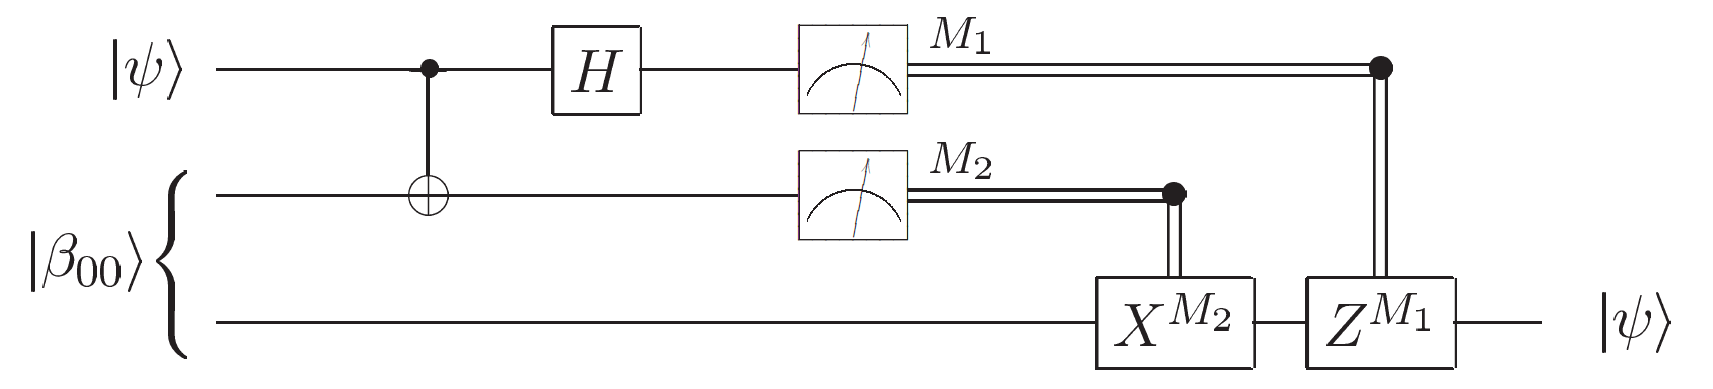
\includegraphics[width=0.48\textwidth]{images/Teleport_general.png}
	\caption{General teleportation protocol circuit. Here the $\ket{\Phi^+}$ Bell-state is denoted as $\ket{\beta_{00}}$.  \cite{nielsen10_quant}}
	\label{fig:telgen}
\end{figure}
Subsequently, a CNOT gate is applied to the second qubit and a Hadamard gate to the first qubit. Now the first and second qubit will be measured in the Z-basis, with the measurement results being $M_1$ and $M_2$, respectively. A X- and/or Z-gate is applied to the third qubit depending on the measurement outcome. If $M_1 = +1$ a Z-gate will be applied and if $M_2 = +1$ a X-gate will be applied. This will result in the state $\ket{\psi}$ being teleported to the third qubit.

However, to know if the state $\ket{\psi}$ is properly transported, the third qubit must be measured. Unfortunately, it is not possible (yet) to apply a gate after a measurement on the used devices. So, we will have to resort to post measurement techniques, as the gates cannot be applied to the third qubit. The circuit that is send to the devices is presented in figure \ref{fig:telcir}.
\begin{figure}[h]
	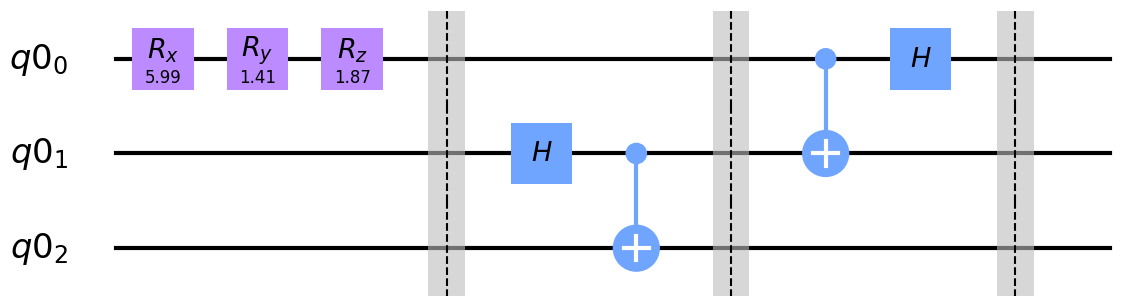
\includegraphics[width=0.48\textwidth]{images/teleport_circuit.png}
	\caption{Teleport circuit used for the measurements. (The operators on the first qubit were randomized every run.)}
	\label{fig:telcir}
\end{figure}
As one can easily see the gates on the third qubit are absent. To account for this, a Pauli-X or Pauli-Z matrix is applied to the final state on the third qubit, after the measurement. Which works similar to the general protocol: if $M_1 = +1$ a Pauli-Z matrix will be applied and if $M_2 = +1$ a Pauli-X matrix will be applied. This will, in post measurement, result in the state $\ket{\psi}$ being teleported to the third qubit.

\subsection{Grover's search algorithm}
The Grover search algorithm can find an input given to a black box with a high likeliness. In our case, the input that is given is a unitary 4x4 diagonal matrix, with three values being +1 and one being -1. The algorithm can find which one of the numbers on the diagonal is -1. The circuit that is used in the measurements is presented in figure \ref{fig:grocir}.
\begin{figure}[h]
	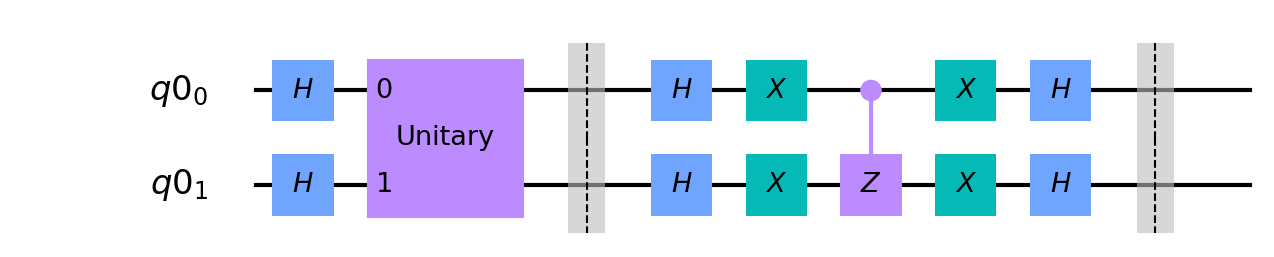
\includegraphics[width=0.48\textwidth]{images/grover_circuit.png}
	\caption{Grover's search algorithm circuit used for the measurements. (The position of the -1 value is randomized every run.)}
	\label{fig:grocir}
\end{figure}
For explanatory reasons, let us choose the unitary matrix to be:
\begin{equation*}
U = 
  \begin{bmatrix}
1 & 0 & 0 & 0 \\
0 & 1 & 0 & 0 \\
0 & 0 & 1 & 0 \\
0 & 0 & 0 & -1 
\end{bmatrix}
\end{equation*} 
$U$ is randomized for every run of the circuit on a device or simulator. The two qubit will both start in the $\ket{0}$ state. After the application of the Hadamard gates the total state will be: $\ket{\Psi} = \frac{1}{2}\left(\ket{00}+\ket{01}+\ket{10}+\ket{11}\right)$. Now $U$ is applied giving: $\ket{\Psi} = \frac{1}{2}\left(\ket{00}+\ket{01}+\ket{10}-\ket{11}\right)$.
The part after the unitary in figure \ref{fig:grocir} is important for the Grover's search algorithm and does an inversion about the mean. This inverts the constants multiplied with each state around the mean of the total. In this case the mean is $\frac{3\cdot\frac{1}{2}-\frac{1}{2}}{4} = \frac{1}{4}$. Inverting $\frac{1}{2}$ about the mean, means that it will become 0. For $-\frac{1}{2}$ it will become 1, thus making $\ket{11}$ the only state left. Measuring this will result in $M_1 = M_2 = +1$. This result is related to where in $U$ the -1 value is positioned and in this case the result shows it is in the bottom right corner (where we positioned -1 in the first place).

\subsection{Entanglement swap}







\section{Results} In the following sections we will discuss some key results;
for a more complete look at the output of the scripts, we ask that you please
consult the Appendices.

\subsection{Teleportation} The main result of the teleportation protocol is
summarized in Fig. \ref{fig:teleport_histogram}. The ideal simulation fidelities
are all within statistical error of unity, an important check to ensure that the
state, reconstructed through tomography, and post-measurement selection scheme
both are working as expected. The Noisy Simulator is modelled using the
single-qubit errors, CNOT errors and a model of readout error in each backend
\cite{qiskit_org}. As we will continue to see with the other circuits, the noise
model overestimate the performance of the backend, but interestingly in this
case, for the Melbourne device, we find that the noise model almost matches that
of the device.

The noise model captures the error in the Burlington device much less
accurately. We would expect that Burlington would perform almost as well as
Yorktown from the estimates on the noisy simulator, but in fact it performs the
worst of the three. We suspect, as will be described in more detail below, that
this is a consequence of the number of gates needed to implement the circuit on
the real device.

\begin{figure}[h] \centering
	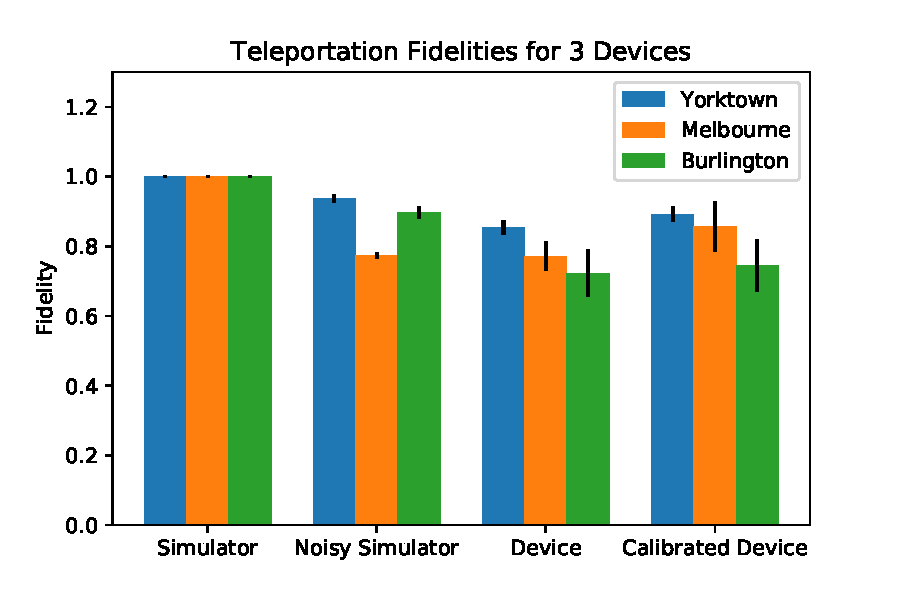
\includegraphics[width=0.48\textwidth]{images/results/teleport_histogram.pdf}
	\caption{Fidelity results for the Teleportation protocol. Error bars are
		estimated by taking the variance over 15 runs of 8,192 shots each (a total of
		122,880 shots). All simulation fidelities are within statistical error of
		unity.}
	\label{fig:teleport_histogram}
\end{figure}
In order to check the readout calibration, it is useful to compare Pauli sets of
the different outcomes, which we can see in Fig. \ref{fig:tele_paulis}.
\begin{figure}
  \begin{subfigure}{.5\textwidth} \centering % include first image
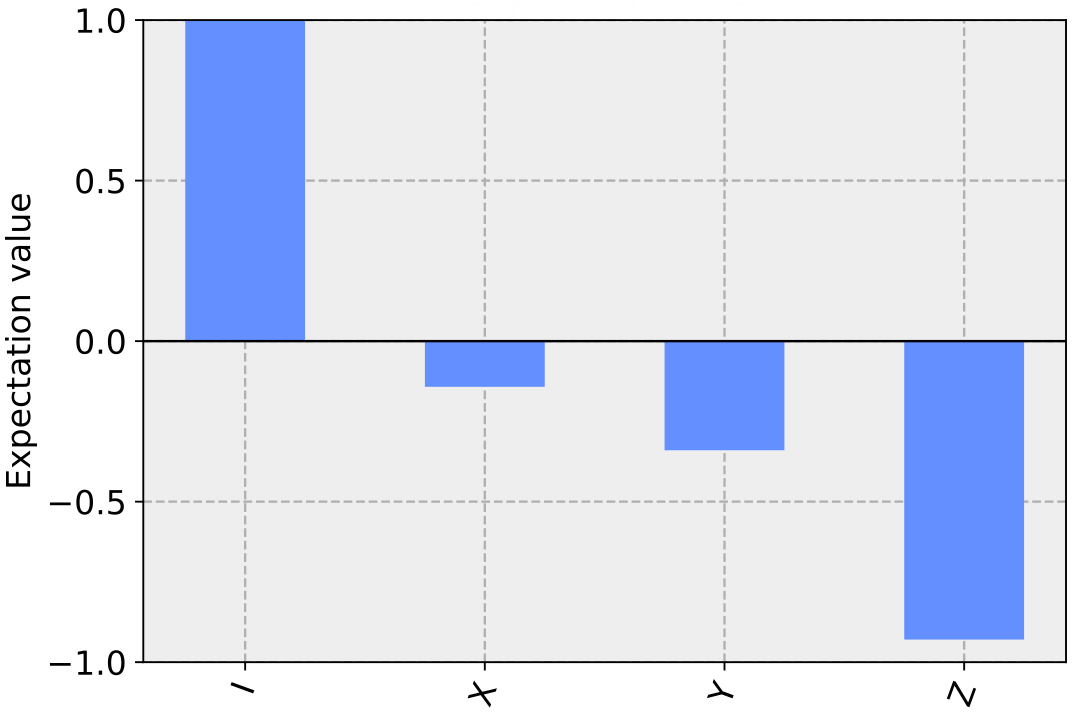
\includegraphics[width=.8\linewidth]{images/results/tele_pauli_sim.png}
    \caption{The expected Pauli set.}
    \label{fig:tele_pauli_sim}
  \end{subfigure} \newline
  \begin{subfigure}{.5\textwidth} \centering % include second image
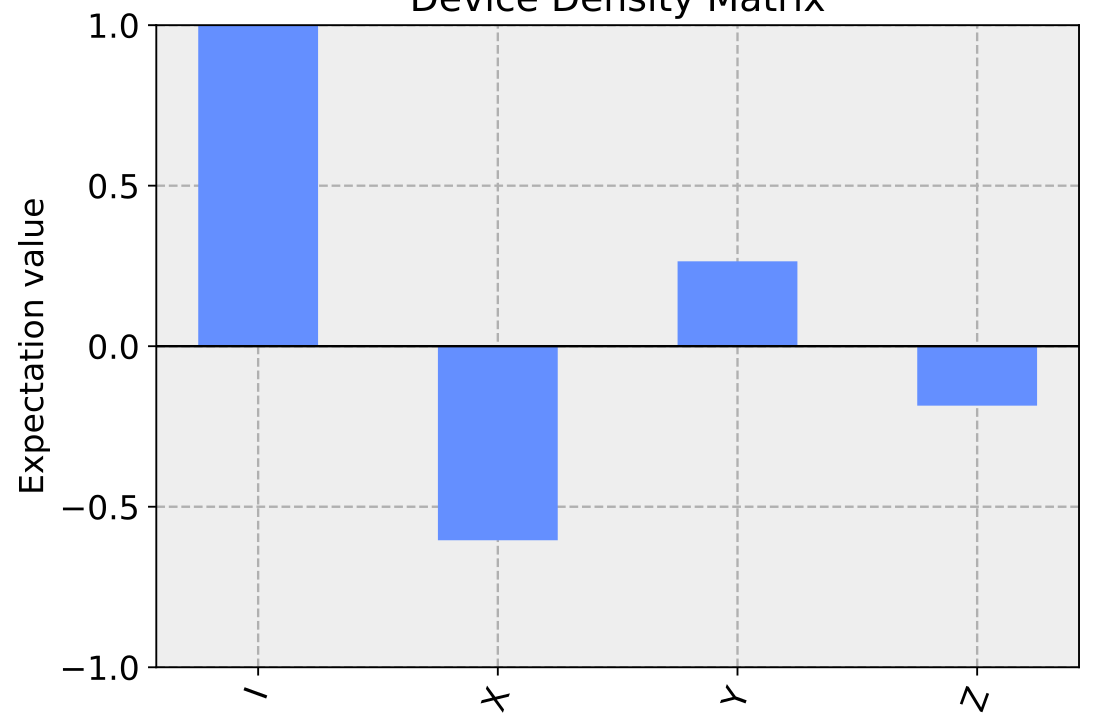
\includegraphics[width=.8\linewidth]{images/results/tele_pauli_dev.png}
    \caption{The output Pauli set for the device.}
    \label{fig:tele_pauli_dev}
  \end{subfigure} \newline
  \begin{subfigure}{.5\textwidth} \centering % include second image
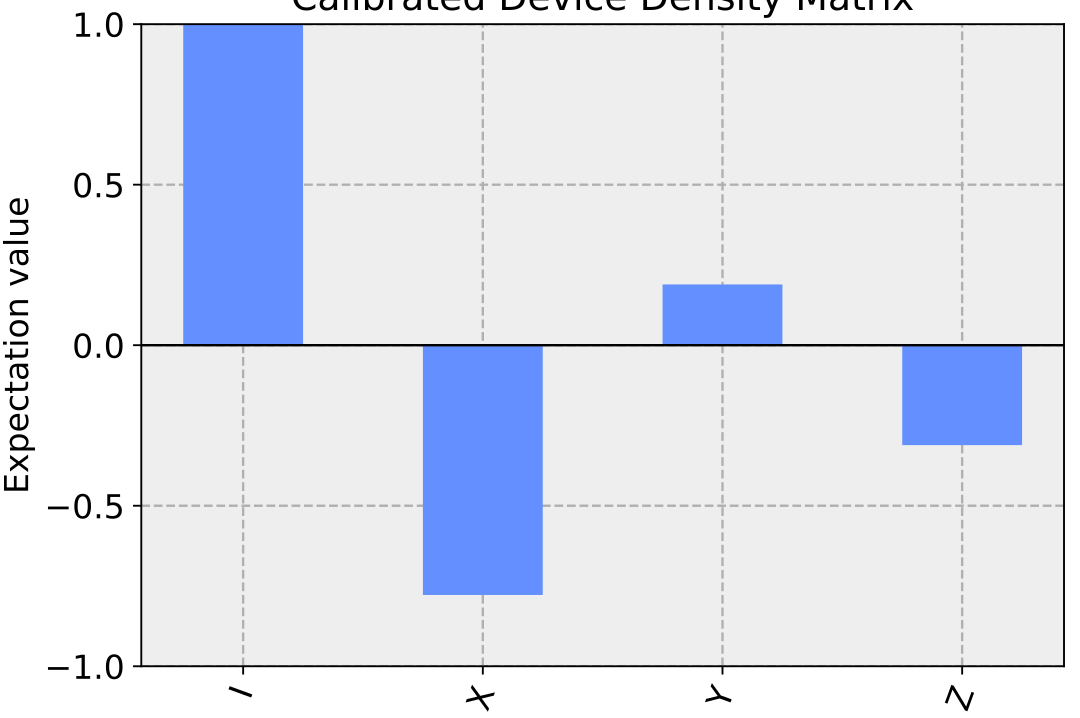
\includegraphics[width=.8\linewidth]{images/results/tele_pauli_cal.png}
    \caption{The calibrated device Pauli set.}
    \label{fig:tele_pauli_dev}
  \end{subfigure}
  \caption{The expectation values match those we expect after calibrating for
readout error. Errors in measurement contribute greatly to the low fidelity of
our final states. The type of correction seen in the figures above accounts for
the increased fidelity for the calibrated device in Fig.
\ref{fig:teleport_histogram}. Data plotted here is taken for 8192 shots on the
Melbourne backend.}
  \label{fig:tele_paulis}
\end{figure}


This thing here is to test a full size picture don't delete.
\begin{figure*}
  \centering
  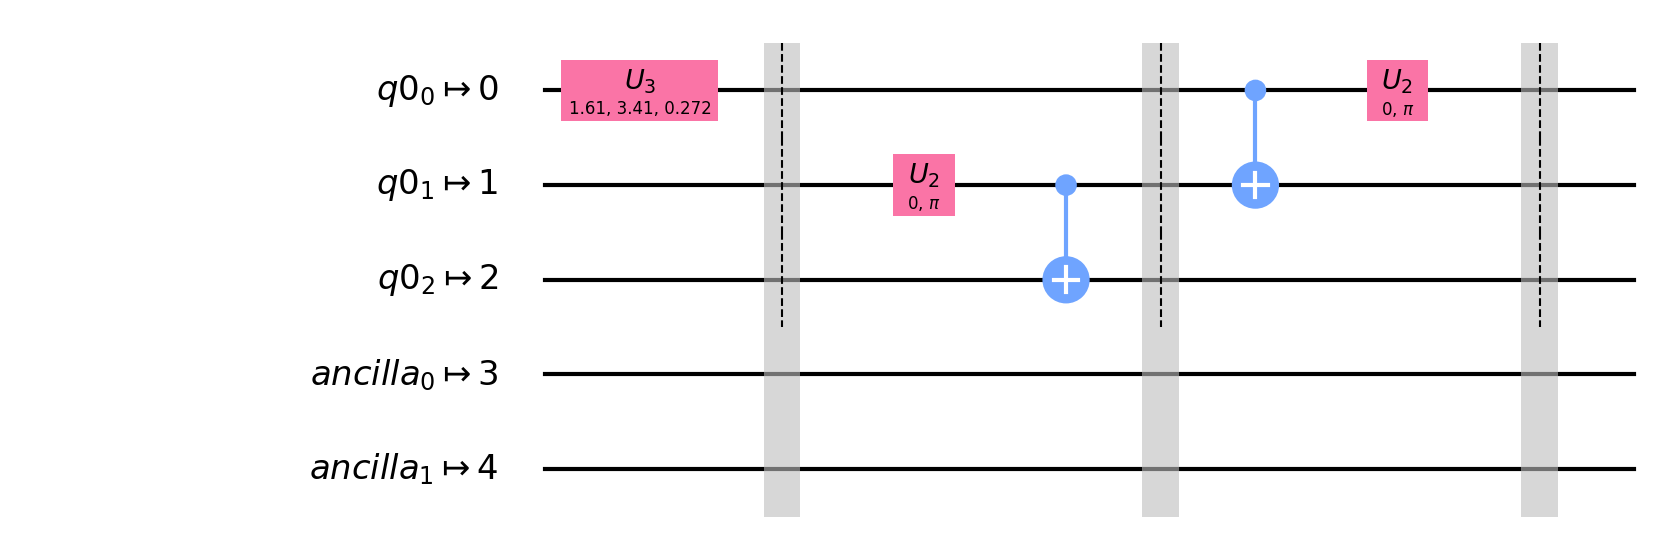
\includegraphics[width=\textwidth]{images/teleport_ibmqx2.png}
  \caption{The most densely connected 5-qubit device at IBM Q. As we will see,
    equally as important as the single-qubit and CNOT error rates is the degree of
    connectivity in a device. Figure from \cite{ibmq_yorktown}.}
  \label{fig:yorktown_connections}
\end{figure*}

\subsection{Entanglement Swapping}
As for teleportation we first look at the main result of the entanglement swapping circuit in Fig. \ref{fig:swap_histogram}. The fidelity measurements are done with a random generated state and a $\ket{\Phi^+}$ Bell-state instead of the regular entanglement swapping circuit where we only swap Bell-states. Again we see that the simulation fidelities are 1 within statistical error, which means that the swapping of initial Bell-states are done correctly using tomography to construct the final state, and post-measurement selection to transform specified results to specific basis. As we expected fidelities from the noisy simulator are much better than results from all the devices. The main difference between teleportation is the fact that Burlington's performance is worse while the other devices give similar (or slightly worse) fidelities. We could predict this behavior since the circuit uses more qubits and hence the total error (due to operations and the qubits themselves) will be more significant. Also note that using the two state tomography method (see Theory) results in an overall improvement of the fidelity. From this phenomena we can conclude that a significant part of the error is due to readout error.   
\begin{figure}[h] \centering
	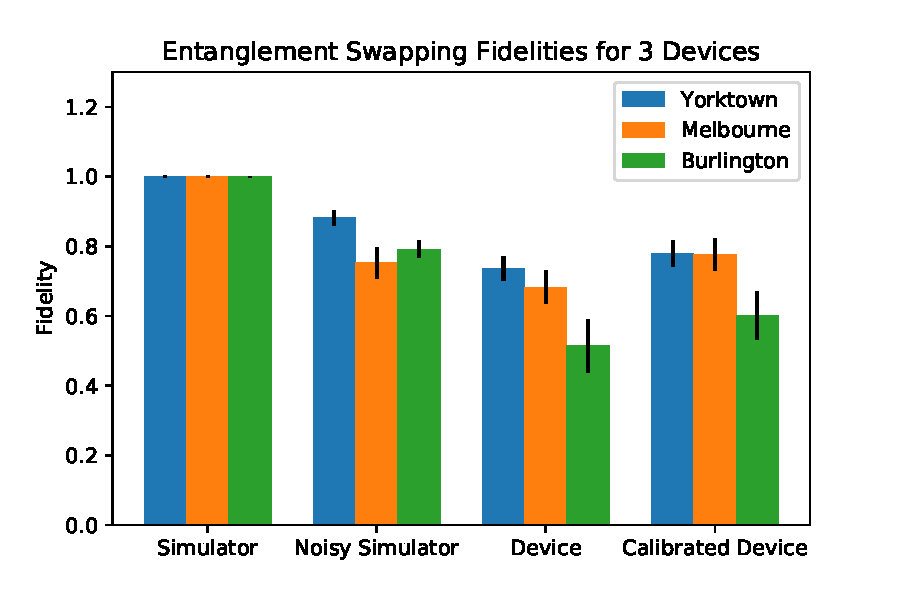
\includegraphics[width=0.48\textwidth]{images/results/swap_histogram.pdf}
	\caption{Fidelity results for the Entanglement Swapping protocol. Error bars are
		estimated by taking the variance over 15 runs of 8,192 shots each (a total of
		122,880 shots).}
	\label{fig:swap_histogram}
\end{figure}

In order to check the readout calibration, it is useful to compare Pauli sets of
the different outcomes, which we can see in Fig. \ref{fig:tele_paulis}.

\begin{figure}
	\begin{subfigure}{.5\textwidth} \centering % include first image
		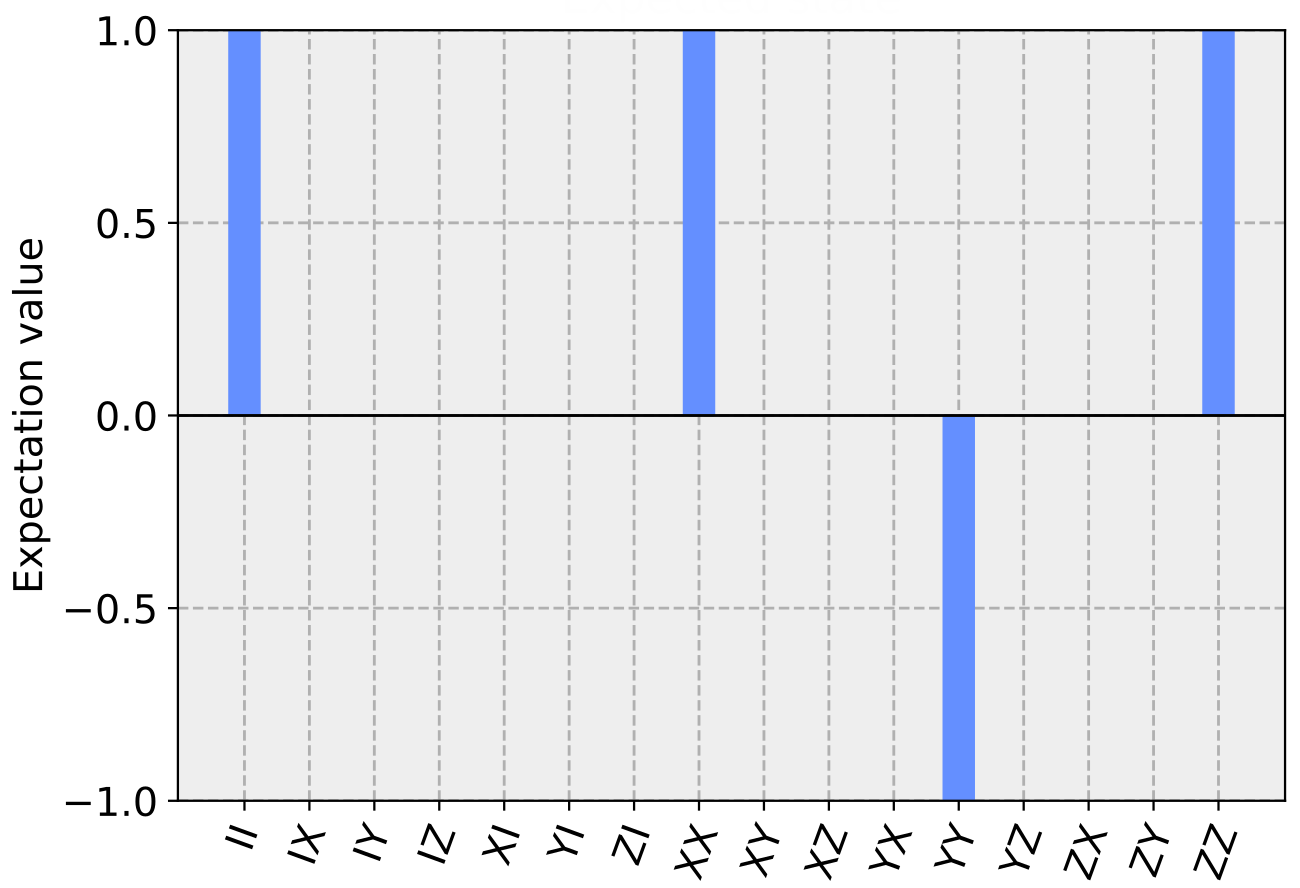
\includegraphics[width=.8\linewidth]{images/results/swap_pauli_sim.png}
		\caption{The expected Pauli set.}
		\label{fig:swap_pauli_sim}
	\end{subfigure} \newline
	\begin{subfigure}{.5\textwidth} \centering % include second image
		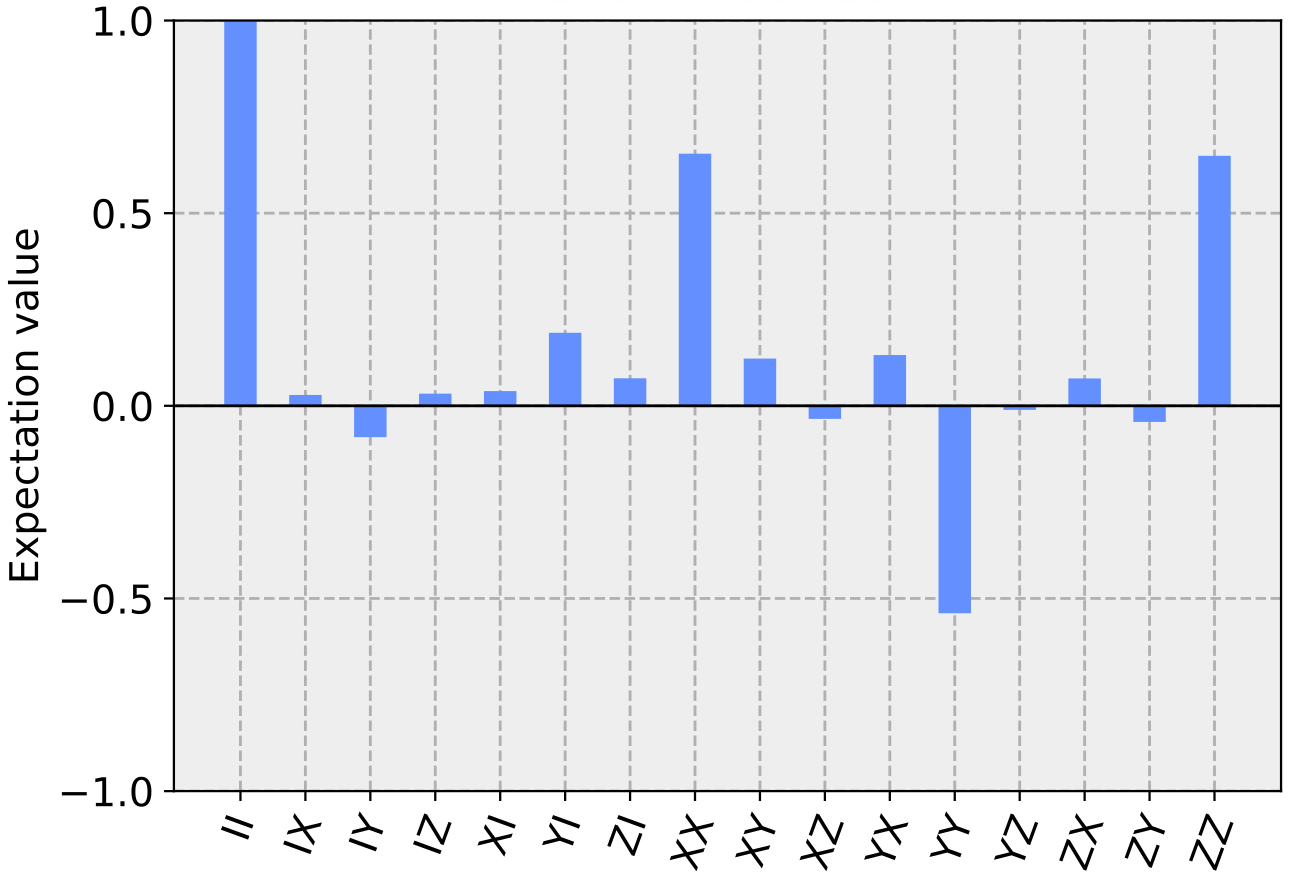
\includegraphics[width=.8\linewidth]{images/results/swap_pauli_dev.png}
		\caption{The output Pauli set for the device.}
		\label{fig:swap_pauli_dev}
	\end{subfigure} \newline
	\begin{subfigure}{.5\textwidth} \centering % include second image
		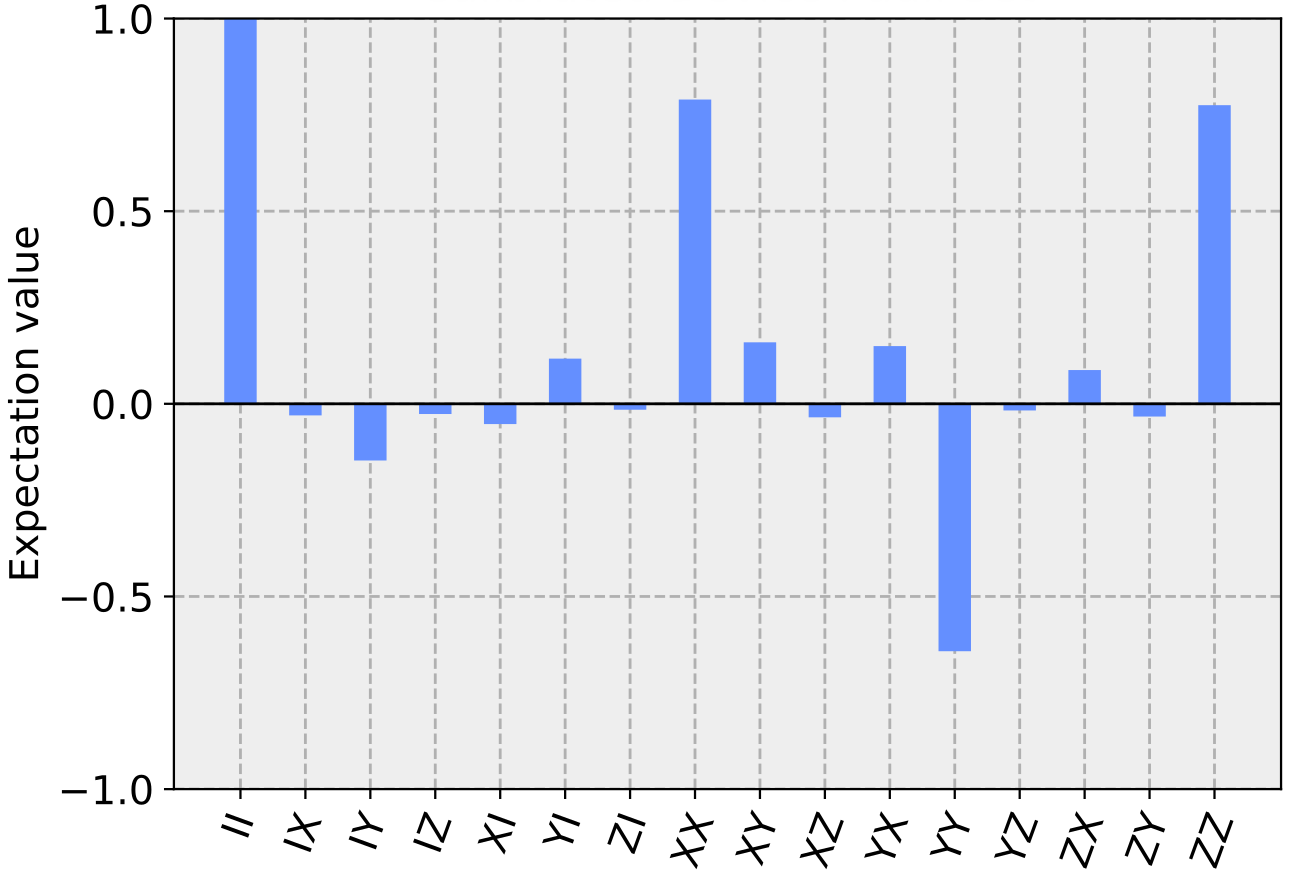
\includegraphics[width=.8\linewidth]{images/results/swap_pauli_cal.png}
		\caption{The calibrated device Pauli set.}
		\label{fig:swap_pauli_dev}
	\end{subfigure}
	\caption{ The type of correction seen in the figures above accounts for
		the increased fidelity for the calibrated device in Fig.
		\ref{fig:swap_histogram}. Data plotted here is taken for 8192 shots on the
		Melbourne backend.}
	\label{fig:tele_paulis}
\end{figure}








\subsection{Entanglement Purification}
\subsection{Grover's Algorithm}


%%% Local Variables:
%%% mode: latex
%%% TeX-master: "report"
%%% End:

\section{Conclusion}

Our research project was mainly focused on the fidelities of different circuits and if we were able to improve those for readout error using state tomography on various circuits. We conclude that we succeeded in recreating the final states using the post measurement method (except for the Grover circuit), since the simulator fidelities for the four circuits are approximately 1. The noisy simulator overestimated the device results for each circuit, and the error correction improves the fidelity for all circuits.  
%%% Local Variables:
%%% mode: latex
%%% TeX-master: "report"
%%% End:

%	REFERENCE LIST
\printbibliography

\section*{Acknowledgements}
We acknowledge use of the IBM Q for this work. The views expressed are those of the authors and do not reflect the official policy or position of IBM or the IBM Q team.

%%% Local Variables:
%%% mode: latex
%%% TeX-master: "report"
%%% End:

% ----------------------------------------------------------------------------------------
\end{document}